
\section{Design and Implementation}

In this section we begin with a system overview of \texttt{Parikshan}. 
We then explain how it inserts test cases, into the test harness, and finally we explain how a user can use the \texttt{Parikshan} api to insert test cases in the test harness.

\begin{figure*}[t]
  \begin{center}
    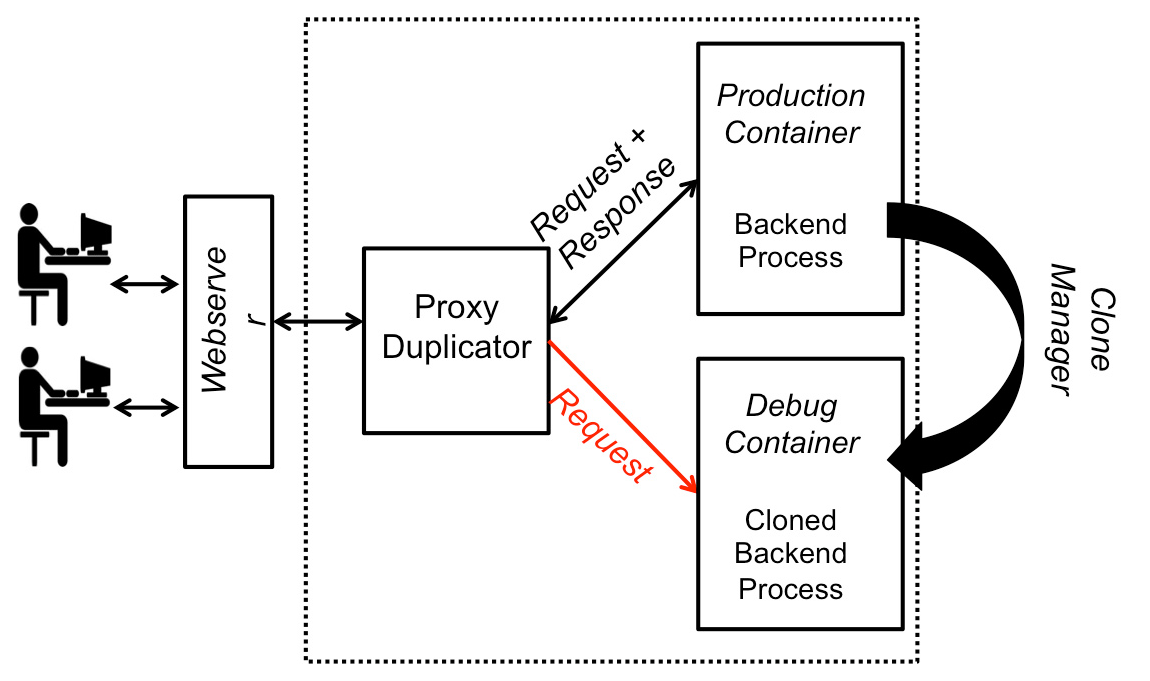
\includegraphics[width=0.8\textwidth]{figs/workflow2.eps}
    \caption{Workflow}
    \label{fig:Backend wrapped around with Parakishan Run-time}
  \end{center}
\end{figure*}


\subsection{System Overview}

Figure 1 shows, a simple 2 tier production model with 


\subsubsection{How does clone manager work?}

While the focus of our work is not to support VM/Container migration, or to make changes to the hypervisor, we need to tweak the way typical hypervisors offer live migration for our purposes.
Before moving further we fish to clarify that instead of the typical live migration supported by hypervisors, \textit{Parikshan} requires a clone of the production container. 
In contrast with live migration, where a container is copied to a target destination, and then the original container is destroyed, the cloning process requires both containers to be actively running, and be still attached to the original network.
This cloning requires some tweaking, and modification in both how compute migration is handled, and especially how the network migration is handled. 

To understand cloning in our context, one must first understand how live migration works. 
Live migration refers to the process of moving a running virtual machine, guest os or container from one host node(physical machine) to another, without disconnecting any client or process running within the machine. 
There are several variants of live migration, some of which require a short suspend time, while others are able to seamlessly transfer without any noticeable down-time by the user.
In general the process involves the following steps: (1) Firstly, the copy is initiated by a pre-copy memory migration, where the underlying hypervisor copies all the memory pages from the source to the destination. (2) Secondly, 
